%------------------- Hip Bracket -------------------%
\subsection{Hip Bracket} \label{subsec:hipbracket}

%------------------------------ Inputs and Outputs ------------------------------%
\subsubsection{Inputs and Outputs}
This section is focused on the analysis of the hip bracket, which is the assembly holding the leg (at the hip control shaft) and attaching it to the chassis. Due to the required range of movement of the leg, this bracket may be quite high. Thus this analysis will take its height and all the forces applied to it and calculate the required thickness of the bracket to prevent failure. 

%------------------------------ CONSTANTS and Assumptions ------------------------------%
\subsubsection{Constants, Parameters and Assumptions}
The safety factor chosen for this part is 2.0 as it is not moving and is merely a structural part. 
The biggest consideration for this bracket is bending at its lower corners in the direction of its thickness, as the bracket will be quite high. Thus, only this stress calculation is performed. 

%------------------------------ Materials ------------------------------%
\subsubsection{Material Selection}
The chosen material is aluminum 6061-T6 as it is marine grade, strong and lightweight. Its yield strength is of about 276 MPa \cite{matweb_aluminum_nodate}.

%------------------------------ Free-Body Diagram ------------------------------%
\subsubsection{Free-Body Diagram}
The following figure shows the various forces applied on the hip bracket and the point being analysed for bending. 

\begin{figure}
    \centering
    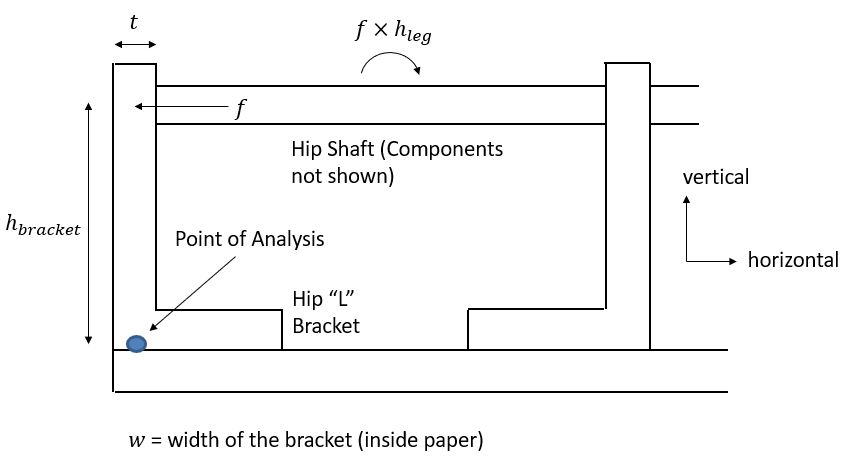
\includegraphics[width=\textwidth]{4_Analysis/img/HipBracket/HipBracket.JPG}
    \caption{Hip Bracket - Bending Stress}
    \label{fig:hipbracket}
\end{figure}

where values of $f$ and $h_{leg}$ are as described in Figure \ref{fig:shaft_hip_friction}, and their product is the moment created by friction at the foot.

%------------------------------ Stress Analysis ------------------------------%
\subsubsection{Stress Analysis}

The equation for the bending moment at the identified critical point ($M_{crit}$) is shown in the following equation. The values are $f=51.7N$, $h_{leg}=190 mm$ and $h_{bracket}=150 mm$ based on required leg movement clearance.

\begin{equation}
    \sum M:\;\;M_{crit}=f\times h_{leg} - f\times h_{bracket}=51.7N (190mm-150mm)=2066.8 Nmm
\end{equation}

Now to find the required minimum thickness of the bracket, the stress equation (for a rectangular cross-section) \cite{juvinall_fundamentals_2012} is used with the chosen safety factor. Values of $SF=2$, $S_y=276 MPa$ and $w=100mm$ are used.

\begin{equation}
    t=\sqrt{\frac{6SF\times M_{crit}}{wS_y}}=\sqrt{\frac{6(2)\times 2066.8Nmm}{100mm (276 MPa)}}=0.9 mm
\end{equation}

%------------------------------ Critical Review ------------------------------%
\subsubsection{Critical Review}
The required value of thickness is quite small as the critical point is quite close to the ground, making the effect of the moment created by friction forces at the foot smaller.

%------------------------------ Parameterization ------------------------------%
\subsubsection{Parameterization}
This component will not be parameterized based on the previous analysis. Instead, the thickness value will be determined by the length of the sleeve bearings for the hip shaft, as they are supported by this bracket. The width of the bracket is based on the size of the harmonic drive and the height is ultimately based on harmonic drives as well, as they affect the required vertical space for the leg range.